\documentclass{beamer-control}
\usepackage{beamer-control-singlefile}
\INCLUDEONLY{Block Diagrams and Transfer Functions}
\begin{document}
\CONCEPT{Block Diagrams and Transfer Functions}

\begin{SUMMARY}
\begin{itemize}
\item Block diagrams
\item Control System Transfer Functions
\item Algebraic Loops
\end{itemize}
\vfill References:
\begin{itemize}
\item \astrom{§9.4}
\item \fullcite{seeler2014-sd}
\end{itemize}
\end{SUMMARY}



\SUBCONCEPT{Block diagrams}

\begin{frame}{Graphical representation of equations}
\framesubtitle{Aka `signal flow graphs' (more or less)}

\vfill
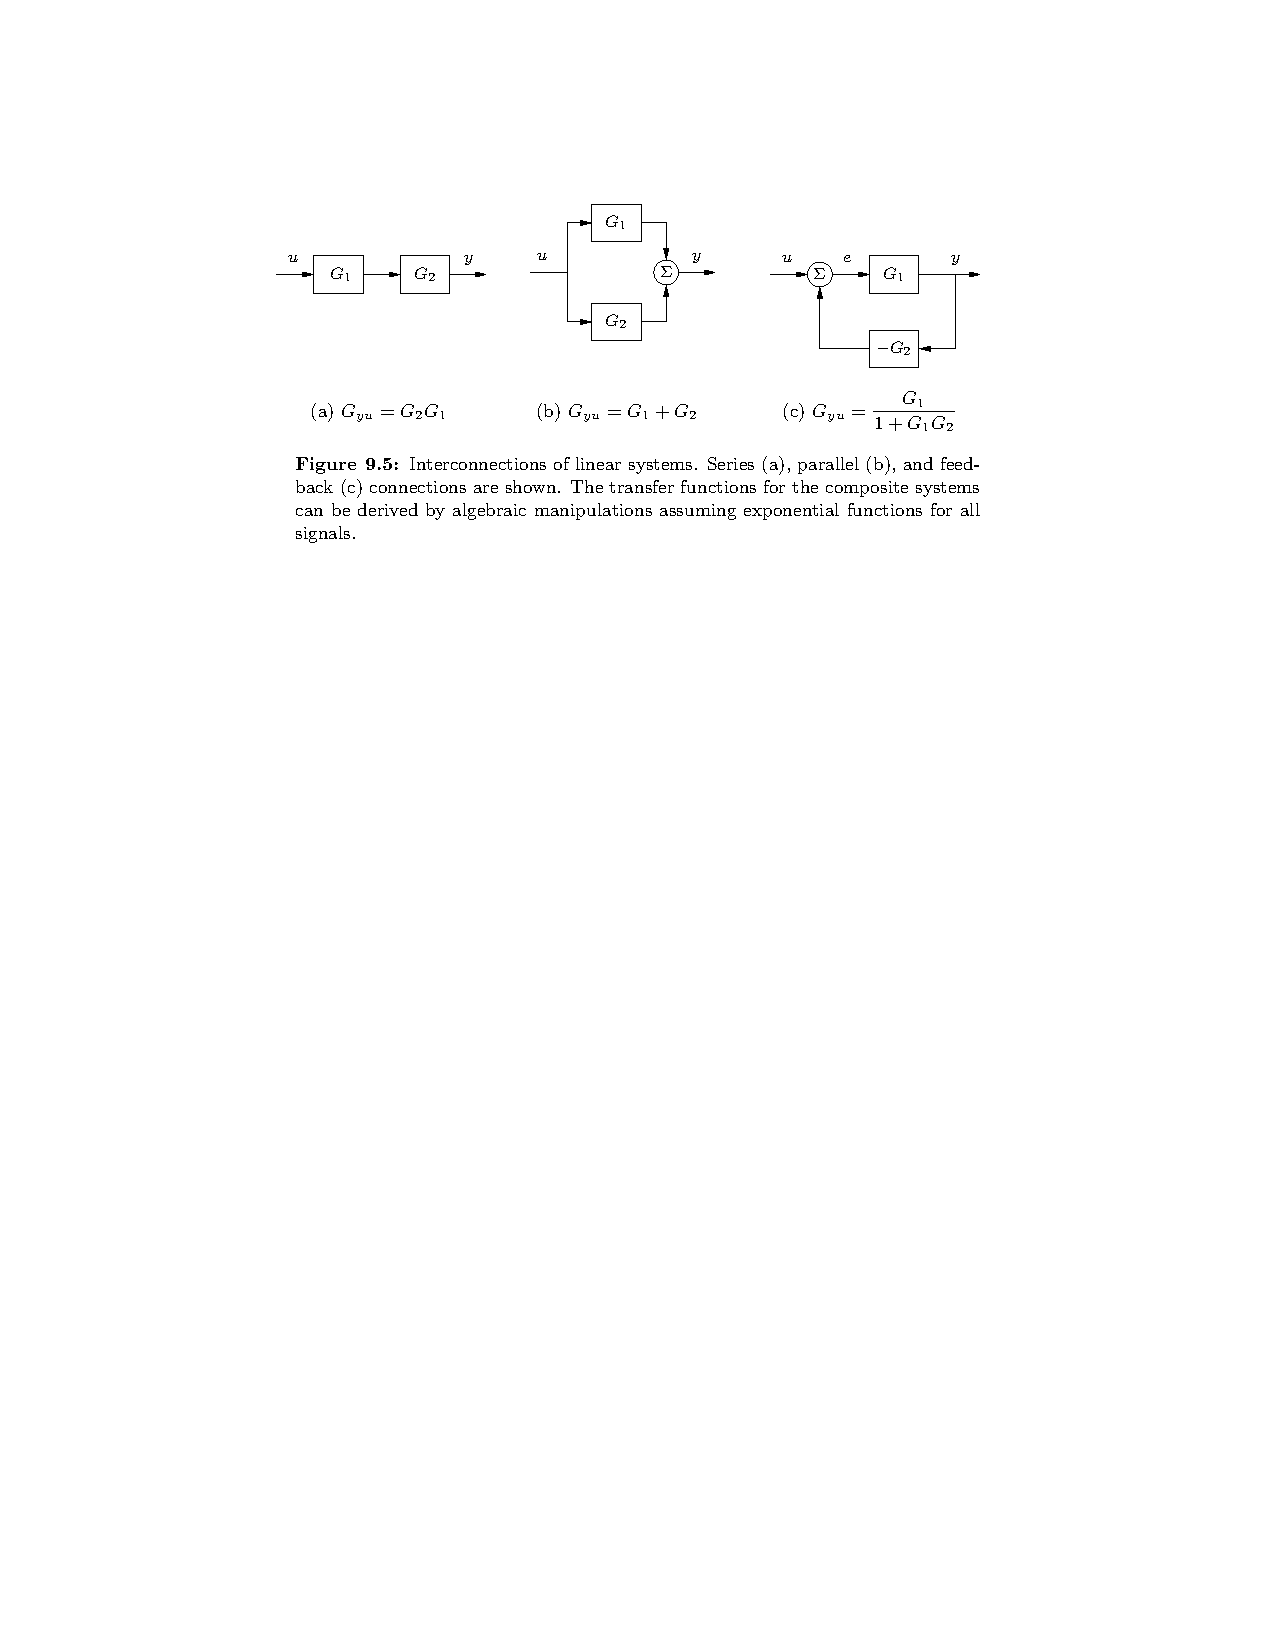
\includegraphics[width=\linewidth]{figure9.5}

\end{frame}

\begin{frame}
\frametitle{What is a block?}
\small

\begin{columns}
\column{0.5\linewidth}
\begin{tikzpicture}[>=Latex, thick, node distance=1cm]
  % Block
  \node[draw, minimum width=25mm, minimum height=10mm, align=center] (block) {`Operator'};
  
  % Input arrow
  \draw[->] 
    ([xshift=-15mm]block.west) -- (block.west)
    node[midway, above] {Input};

  % Output arrow
  \draw[->]
    (block.east) -- ([xshift=15mm]block.east)
    node[midway, above] {Output};
\end{tikzpicture}

\column{0.5\linewidth}
\begin{tikzpicture}[>=Latex, thick, node distance=1cm]
  % Block
  \node[draw, minimum width=25mm, minimum height=10mm, align=center] (block) {$G_{yu}$};
  
  % Input arrow
  \draw[->] 
    ([xshift=-15mm]block.west) -- (block.west)
    node[midway, above] {$u$};

  % Output arrow
  \draw[->]
    (block.east) -- ([xshift=15mm]block.east)
    node[midway, above] {$y$};
\end{tikzpicture}
\bigskip

\begin{tikzpicture}[>=Latex, thick, node distance=1cm]
  % Block
  \node[draw, minimum width=25mm, minimum height=10mm, align=center] (block) {$\Deriv{}{t}$};
  
  % Input arrow
  \draw[->] 
    ([xshift=-15mm]block.west) -- (block.west)
    node[midway, above] {$u$};

  % Output arrow
  \draw[->]
    (block.east) -- ([xshift=15mm]block.east)
    node[midway, above] {$\dot u$};
\end{tikzpicture}
\bigskip

\begin{tikzpicture}[>=Latex, thick, node distance=1cm]
  % Block
  \node[draw, minimum width=25mm, minimum height=10mm, align=center] (block) {$\int \dee t$};
  
  % Input arrow
  \draw[->] 
    ([xshift=-15mm]block.west) -- (block.west)
    node[midway, above] {$\dot u$};

  % Output arrow
  \draw[->]
    (block.east) -- ([xshift=15mm]block.east)
    node[midway, above] {$u$};
\end{tikzpicture}

\end{columns}

\vfill

\end{frame}

\begin{frame}{Deriving the feedback loop}


\end{frame}

\begin{frame}{Block diagram algebra}
\framesubtitle{\minicite{seeler2014-sd}}

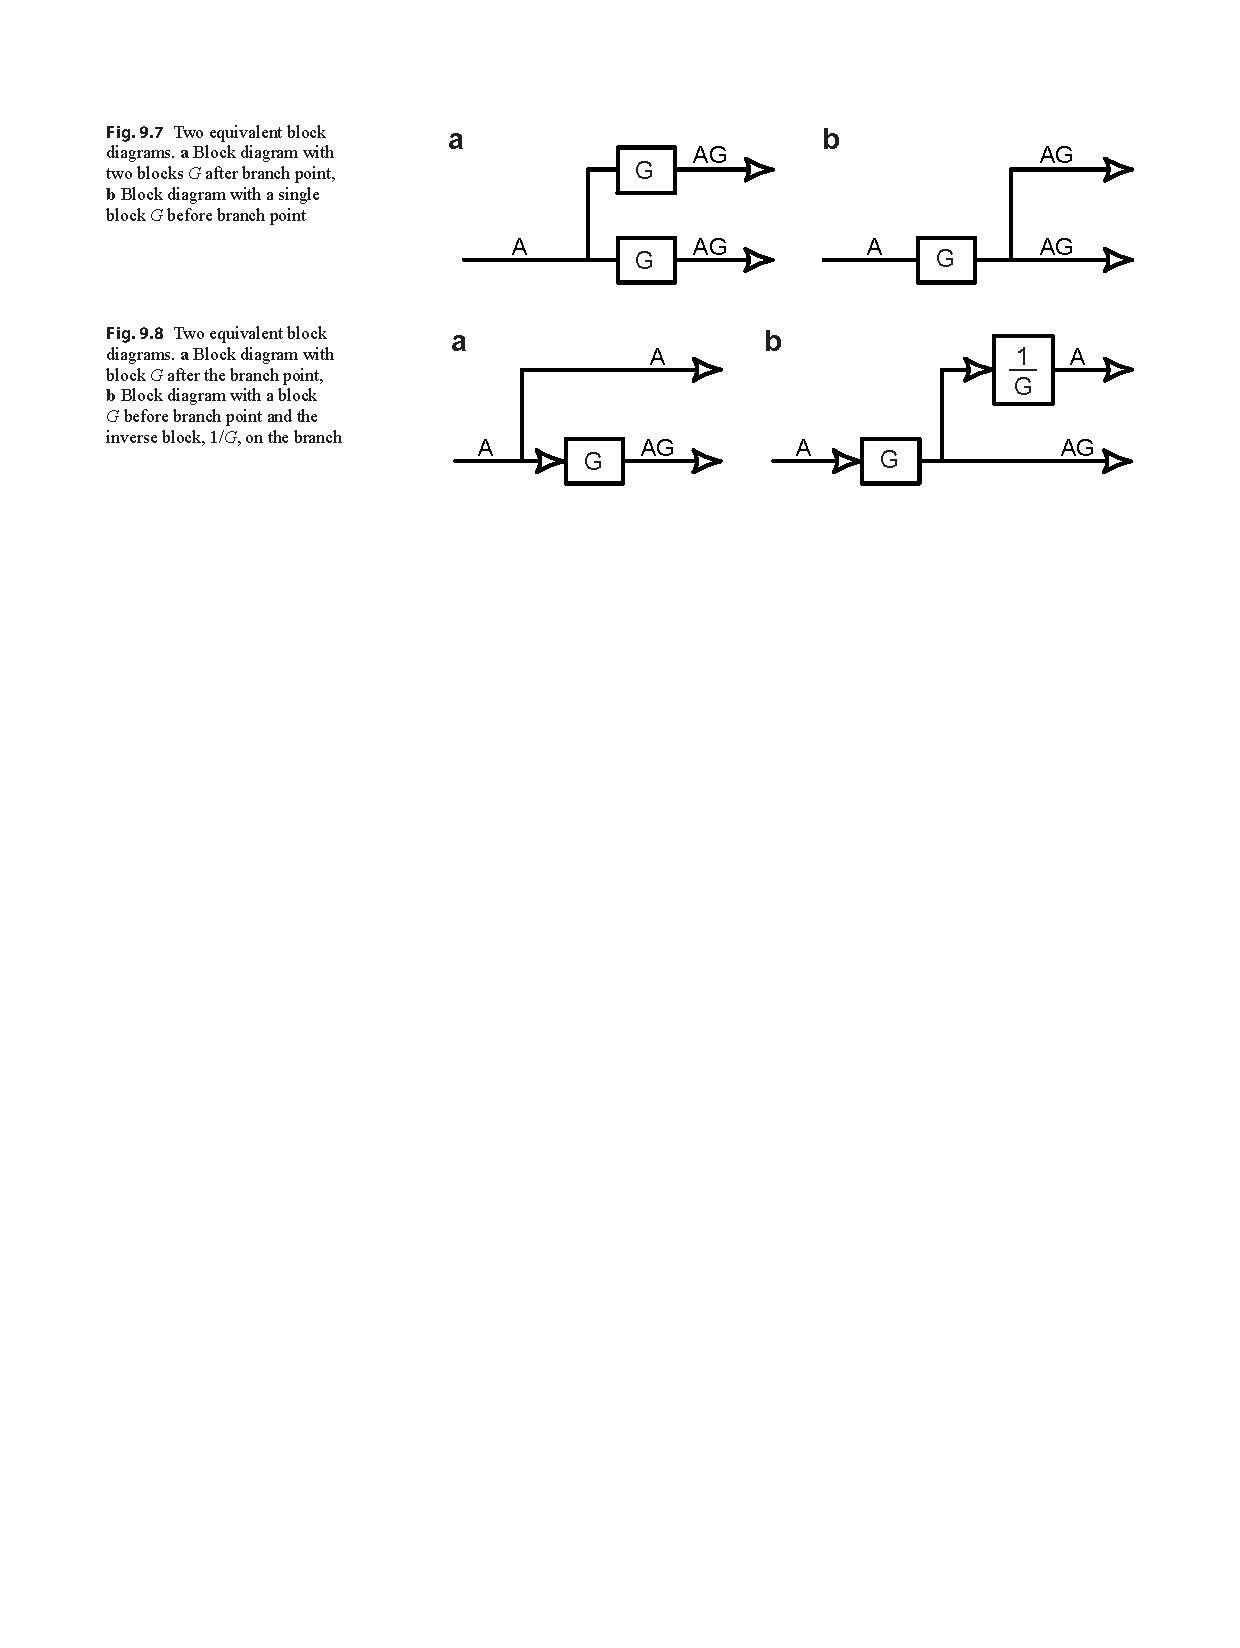
\includegraphics[width=\linewidth]{seeler-fig9.7}

\end{frame}

\begin{frame}
\frametitle{Block diagram rearranging and detangling}
\framesubtitle{\minicite{seeler2014-sd} --- Figs 9.24--9.25}

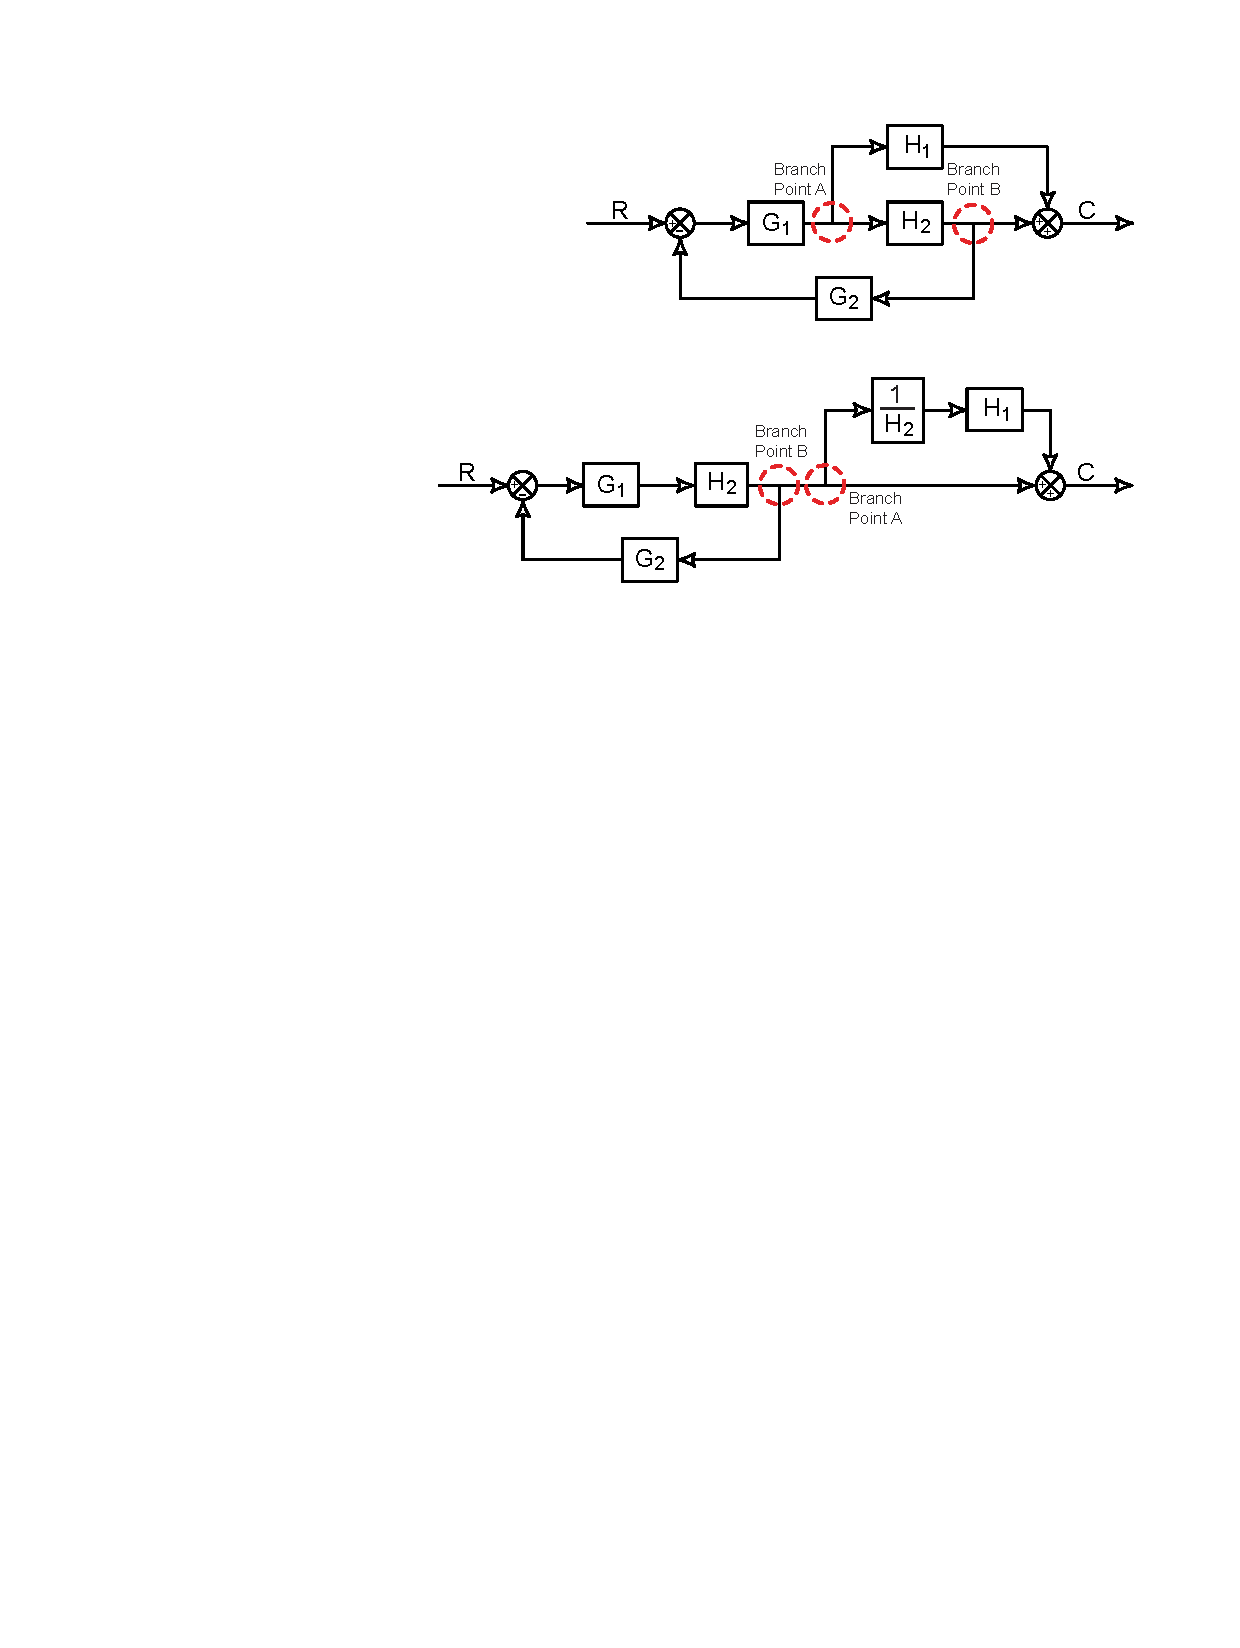
\includegraphics[width=\linewidth]{seeler-fig9.24}


\end{frame}

\SUBCONCEPT{Control System Transfer Functions}

\begin{frame}{Closed loop transfer function}{\AMref{Figures 9.6--9.7}}

\centering
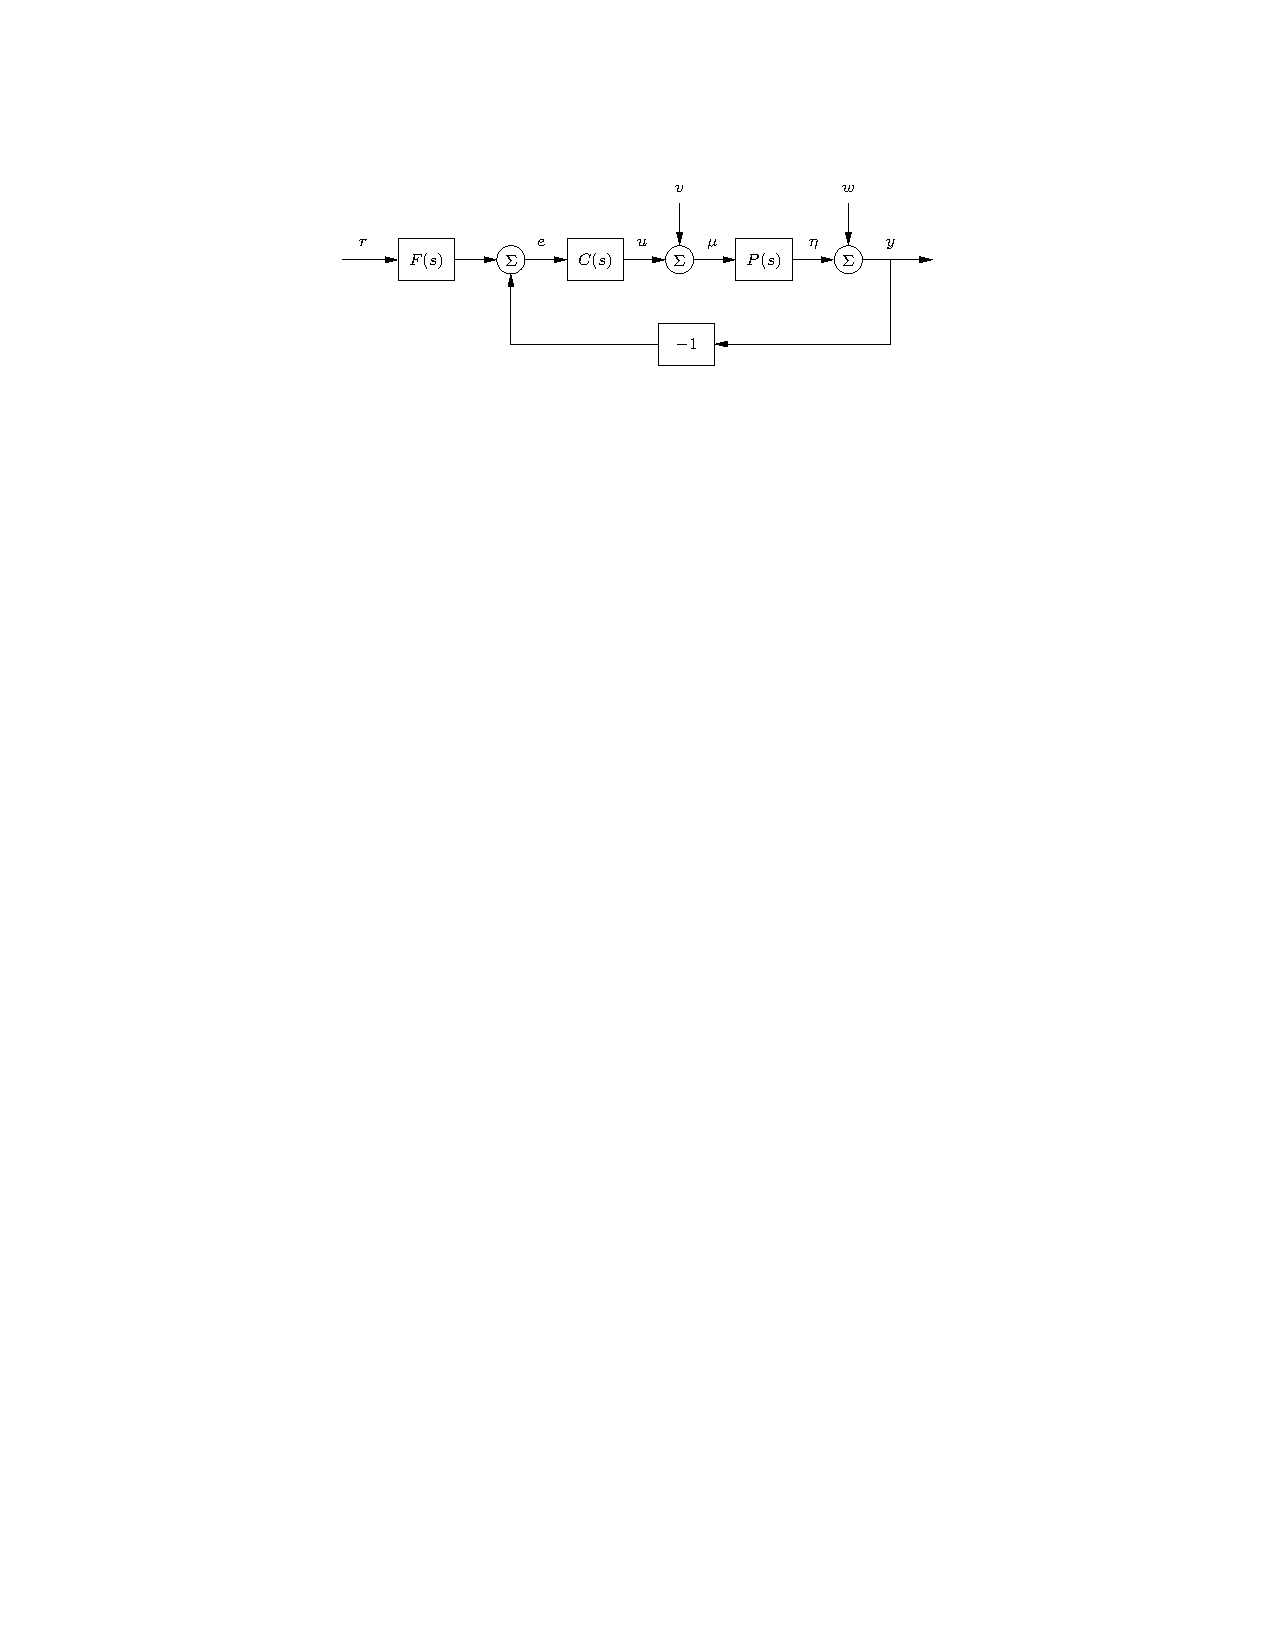
\includegraphics[height=0.4\textheight]{figure9.6}

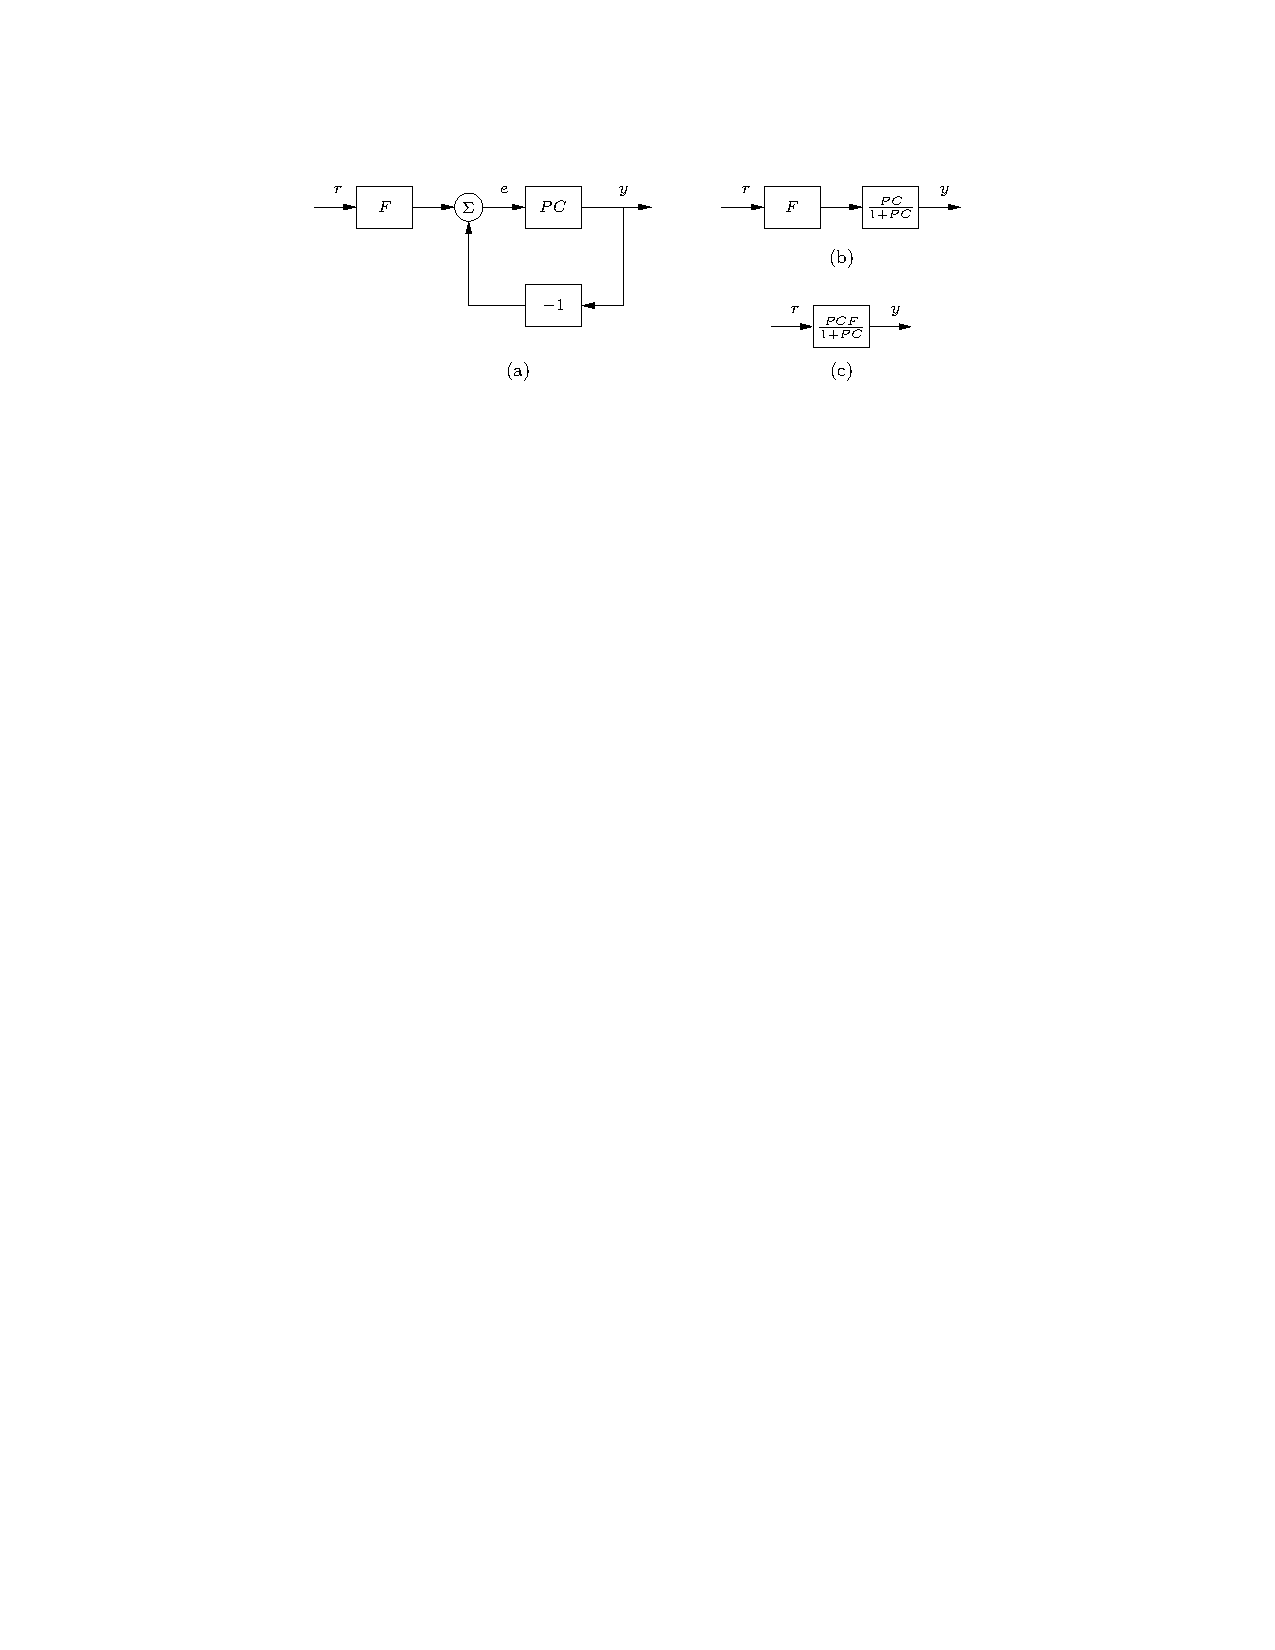
\includegraphics[height=0.4\textheight]{figure9.7}


\end{frame}

\begin{frame}
\frametitle{State space control system block diagram}

\small
\begin{tikzpicture}[>=Latex, thick, node distance=10mm]
  % Nodes
  \node (u) {$u$};
  \node[draw, minimum width=1.2cm, minimum height=1cm, right=of u] (B) {$B$};
  \node[circle, draw, right=of B] (sum) {$\Sigma$};
  \node[draw, minimum width=1.2cm, minimum height=1cm, right=of sum] (int) {$\int$};
  \node[draw, minimum width=1.2cm, minimum height=1cm, right=of int] (C) {$C$};
  \node[right=of C] (y) {$y$};

  % Feedback
  \node[draw, minimum width=1.2cm, minimum height=1cm, above=of int] (A) {$A$};

  % Connections
  \draw[->] (u) -- (B);
  \draw[->] (B) -- (sum);
  \draw[->] (sum) -- (int);
  \draw[->] (int) -- (C);
  \draw[->] (C) -- (y);

  % Feedback arrow starts after integrator
  \draw[->] (int.east) ++(0.5,0) |- (A);
  \draw[->] (A) -| (sum.north);

  % Label x
  \node at ($(int)!0.5!(C)$) [below] {$x$};
  \node at ($(sum)!0.5!(int)$) [below] {$\dot x$};
 
\end{tikzpicture}

\end{frame}

\begin{frame}
\frametitle{State space controller with estimator --- equations }

\begin{align}
\Deriv{x}{t} &= Ax + Bu, \qquad y = Cx \\
u &= -K \hat x + k_f r \\
\Deriv{\hat x}{t} &= A\hat x + Bu+L(y-C\hat x)
\end{align}

\end{frame}

\begin{frame}
\frametitle{State space controller with estimator --- block diagram}

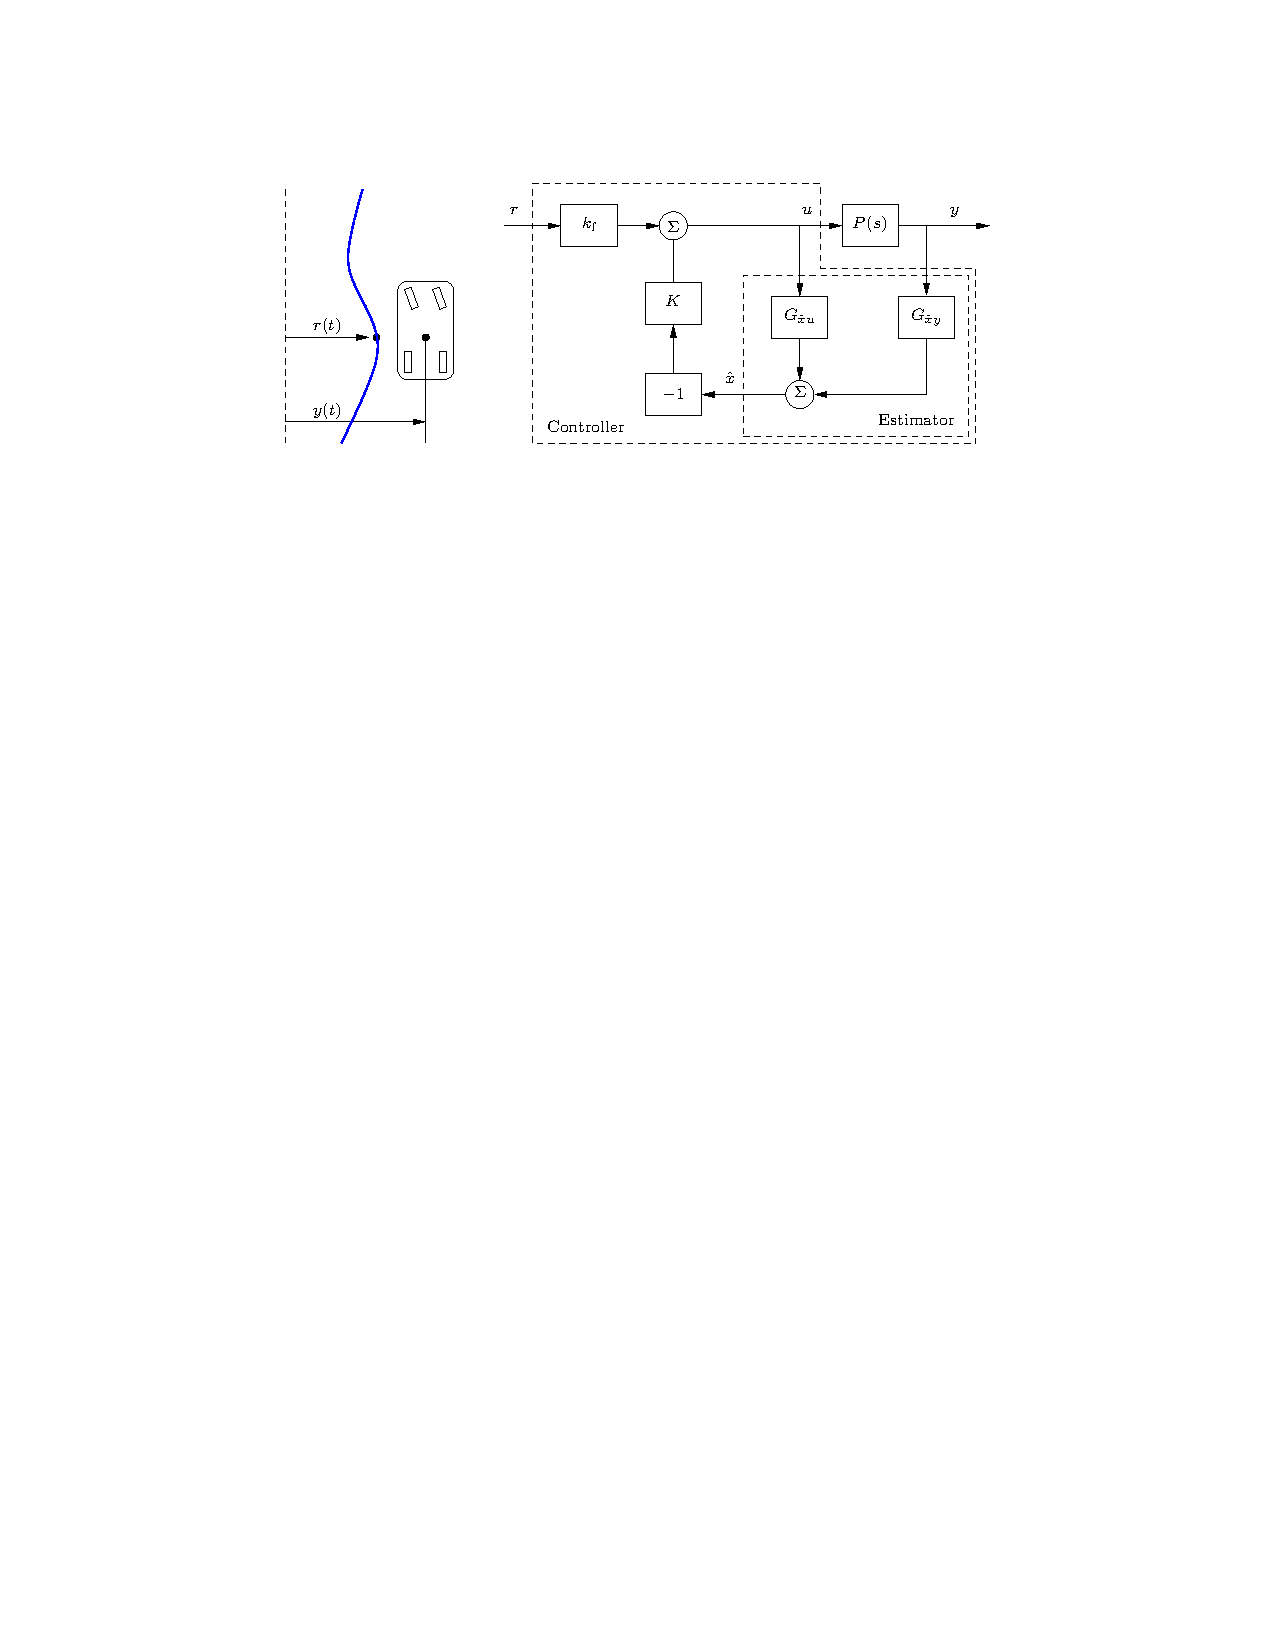
\includegraphics[width=\linewidth]{figure9.8}

\vspace*{0pt plus 1filll}
\begin{align}
G_{yr} &= \frac{P(s) G_{ur}(s)}{1 - P(s) G_{uy}(s)}
\end{align}


\end{frame}

\SUBCONCEPT{Algebraic Loops}

\begin{frame}{Pass through terms cause problems}

Consider proportional feedback based on the state with nonlinear $f(\cdot)$, $h(\cdot)$:
\begin{align}
\Deriv{x}{t} = f(x,-ky), \qquad y = h(x)
\end{align}
Easy to see the differential equations can be numerically solved:
\begin{align}
\Deriv{x}{t} = f(x,-k h(x)) = F(x)
\end{align}
But what to do when
\begin{align}
\Deriv{x}{t} = f(x,-ky), \qquad y = h(x,-ky)
\end{align}
Solving $h(x,-ky)-y=0$ to yield $y=\alpha(x)$ needs an arbitrarily-complex iterative root finder

\end{frame}

\begin{frame}
\frametitle{Matlab/Simulink has an algebraic loop solver}
\framesubtitle{See links to documentation}
\centering
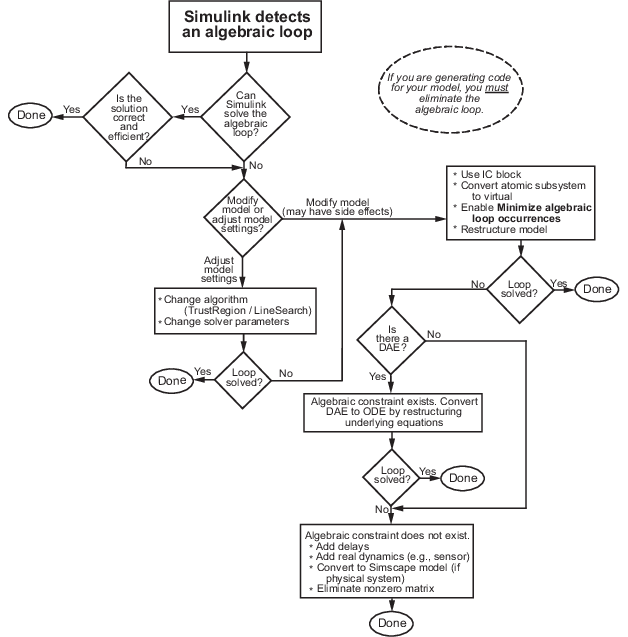
\includegraphics[height=0.8\textheight]{aloop_workflow.png}

\end{frame}


\SUMMARYFRAME
\FINALE

\end{document}
